

\tikzset{every picture/.style={line width=0.75pt}} %set default line width to 0.75pt        

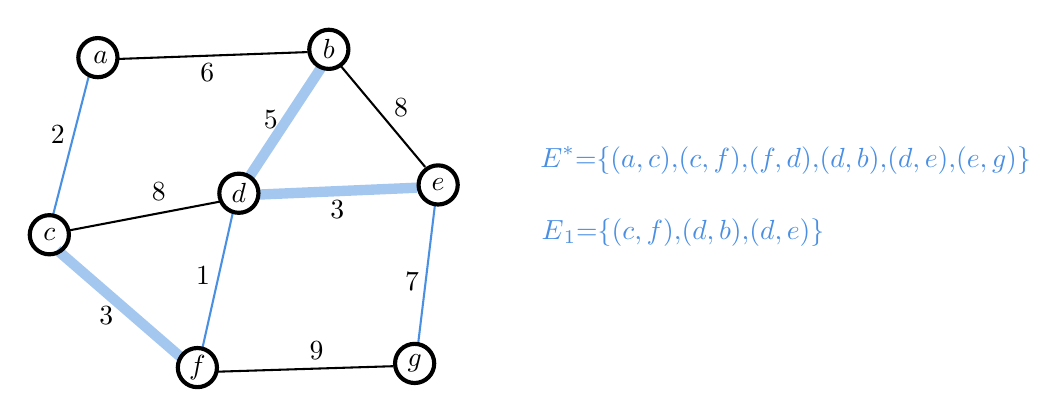
\begin{tikzpicture}[x=0.5pt,y=0.5pt,yscale=-1,xscale=1]
%uncomment if require: \path (0,294); %set diagram left start at 0, and has height of 294

%Straight Lines [id:da823970354045778] 
\draw [color={rgb, 255:red, 0; green, 0; blue, 0 }  ,draw opacity=1 ][line width=0.75]    (237,42) -- (298,115) ;
%Straight Lines [id:da271237396517352] 
\draw [color={rgb, 255:red, 0; green, 0; blue, 0 }  ,draw opacity=1 ][line width=0.75]    (147,263) -- (275,259) ;
%Straight Lines [id:da6657573604931601] 
\draw [color={rgb, 255:red, 74; green, 144; blue, 226 }  ,draw opacity=0.5 ][line width=3.75]    (32,175) -- (122,253) ;
%Straight Lines [id:da31661075744879486] 
\draw [color={rgb, 255:red, 0; green, 0; blue, 0 }  ,draw opacity=1 ][line width=0.75]    (40,161) -- (150,140) ;
%Straight Lines [id:da9969849240959807] 
\draw [color={rgb, 255:red, 74; green, 144; blue, 226 }  ,draw opacity=1 ][line width=0.75]    (55,49) -- (29,150) ;
%Straight Lines [id:da14506071047898028] 
\draw [color={rgb, 255:red, 0; green, 0; blue, 0 }  ,draw opacity=1 ][line width=0.75]    (75,37) -- (213,32) ;
%Straight Lines [id:da8946288202546534] 
\draw [color={rgb, 255:red, 74; green, 144; blue, 226 }  ,draw opacity=0.5 ][line width=3.75]    (223,43) -- (171,122) ;
%Straight Lines [id:da15496081521651384] 
\draw [color={rgb, 255:red, 74; green, 144; blue, 226 }  ,draw opacity=1 ][line width=0.75]    (159,148) -- (137,246) ;
%Straight Lines [id:da2163317830574415] 
\draw [color={rgb, 255:red, 74; green, 144; blue, 226 }  ,draw opacity=1 ][line width=0.75]    (305,143) -- (293,242) ;
%Straight Lines [id:da5391246746067021] 
\draw [color={rgb, 255:red, 74; green, 144; blue, 226 }  ,draw opacity=0.5 ][line width=3.75]    (292,130) -- (177,135) ;

% Text Node
\draw  [line width=1.5]   (307.38, 128) circle [x radius= 14.15, y radius= 14.15]   ;
\draw (307.38,128) node   [align=left] {$\displaystyle e$};
% Text Node
\draw  [line width=1.5]   (61.48, 36) circle [x radius= 14.15, y radius= 14.15]   ;
\draw (55.98,36) node [anchor=west] [inner sep=0.75pt]   [align=left] {$\displaystyle a$};
% Text Node
\draw  [line width=1.5]   (228.38, 30) circle [x radius= 14.15, y radius= 14.15]   ;
\draw (228.38,30) node   [align=left] {$\displaystyle b$};
% Text Node
\draw  [line width=1.5]   (26.38, 164) circle [x radius= 14.15, y radius= 14.15]   ;
\draw (26.38,164) node   [align=left] {$\displaystyle c$};
% Text Node
\draw  [line width=1.5]   (163.38, 134) circle [x radius= 14.15, y radius= 14.15]   ;
\draw (163.38,134) node   [align=left] {$\displaystyle d$};
% Text Node
\draw  [line width=1.5]   (133.38, 260) circle [x radius= 14.15, y radius= 14.15]   ;
\draw (133.38,260) node   [align=left] {$\displaystyle f$};
% Text Node
\draw  [line width=1.5]   (290.38, 257) circle [x radius= 14.15, y radius= 14.15]   ;
\draw (290.38,257) node   [align=left] {$\displaystyle g$};
% Text Node
\draw (25.24,83.06) node [anchor=north west][inner sep=0.75pt]   [align=left] {$\displaystyle 2$};
% Text Node
\draw (133.24,38.06) node [anchor=north west][inner sep=0.75pt]   [align=left] {$\displaystyle 6$};
% Text Node
\draw (227.24,137.06) node [anchor=north west][inner sep=0.75pt]   [align=left] {$\displaystyle 3$};
% Text Node
\draw (179.24,72.06) node [anchor=north west][inner sep=0.75pt]   [align=left] {$\displaystyle 5$};
% Text Node
\draw (98.24,124.06) node [anchor=north west][inner sep=0.75pt]   [align=left] {$\displaystyle 8$};
% Text Node
\draw (60.24,214.06) node [anchor=north west][inner sep=0.75pt]   [align=left] {$\displaystyle 3$};
% Text Node
\draw (130.24,185.06) node [anchor=north west][inner sep=0.75pt]   [align=left] {$\displaystyle 1$};
% Text Node
\draw (273.24,63.06) node [anchor=north west][inner sep=0.75pt]   [align=left] {$\displaystyle 8$};
% Text Node
\draw (212.24,239.06) node [anchor=north west][inner sep=0.75pt]   [align=left] {$\displaystyle 9$};
% Text Node
\draw (281.24,189) node [anchor=north west][inner sep=0.75pt]   [align=left] {$\displaystyle 7$};
% Text Node
\draw (379,98) node [anchor=north west][inner sep=0.75pt]   [align=left] {$\displaystyle \textcolor[rgb]{0.29,0.56,0.89}{E}\textcolor[rgb]{0.29,0.56,0.89}{^{*}}\textcolor[rgb]{0.29,0.56,0.89}{=}\textcolor[rgb]{0.29,0.56,0.89}{\{}\textcolor[rgb]{0.29,0.56,0.89}{(}\textcolor[rgb]{0.29,0.56,0.89}{a,c}\textcolor[rgb]{0.29,0.56,0.89}{)}\textcolor[rgb]{0.29,0.56,0.89}{,}\textcolor[rgb]{0.29,0.56,0.89}{(}\textcolor[rgb]{0.29,0.56,0.89}{c,f}\textcolor[rgb]{0.29,0.56,0.89}{)}\textcolor[rgb]{0.29,0.56,0.89}{,}\textcolor[rgb]{0.29,0.56,0.89}{(}\textcolor[rgb]{0.29,0.56,0.89}{f,d}\textcolor[rgb]{0.29,0.56,0.89}{)}\textcolor[rgb]{0.29,0.56,0.89}{,}\textcolor[rgb]{0.29,0.56,0.89}{(}\textcolor[rgb]{0.29,0.56,0.89}{d,b}\textcolor[rgb]{0.29,0.56,0.89}{)}\textcolor[rgb]{0.29,0.56,0.89}{,}\textcolor[rgb]{0.29,0.56,0.89}{(}\textcolor[rgb]{0.29,0.56,0.89}{d,e}\textcolor[rgb]{0.29,0.56,0.89}{)}\textcolor[rgb]{0.29,0.56,0.89}{,}\textcolor[rgb]{0.29,0.56,0.89}{(}\textcolor[rgb]{0.29,0.56,0.89}{e,g}\textcolor[rgb]{0.29,0.56,0.89}{)}\textcolor[rgb]{0.29,0.56,0.89}{\}}$};
% Text Node
\draw (380,150) node [anchor=north west][inner sep=0.75pt]   [align=left] {$\displaystyle \textcolor[rgb]{0.29,0.56,0.89}{E}\textcolor[rgb]{0.29,0.56,0.89}{_{1}}\textcolor[rgb]{0.29,0.56,0.89}{=}\textcolor[rgb]{0.29,0.56,0.89}{\{}\textcolor[rgb]{0.29,0.56,0.89}{(}\textcolor[rgb]{0.29,0.56,0.89}{c,f}\textcolor[rgb]{0.29,0.56,0.89}{)}\textcolor[rgb]{0.29,0.56,0.89}{,}\textcolor[rgb]{0.29,0.56,0.89}{(}\textcolor[rgb]{0.29,0.56,0.89}{d,b}\textcolor[rgb]{0.29,0.56,0.89}{)}\textcolor[rgb]{0.29,0.56,0.89}{,}\textcolor[rgb]{0.29,0.56,0.89}{(}\textcolor[rgb]{0.29,0.56,0.89}{d,e}\textcolor[rgb]{0.29,0.56,0.89}{)}\textcolor[rgb]{0.29,0.56,0.89}{\}}$};


\end{tikzpicture}

